\documentclass[12pt]{article}

% Set font to Helvetica or Garamond
\usepackage[scaled]{helvet} % For Helvetica font
% \usepackage{Garamond}      % Uncomment this line if you want Garamond font instead

% Set letter spacing (1.15)
\usepackage{microtype} % Automatically handles letterspacing
\SetTracking{encoding=*}{+25} % Slightly increases letterspacing

\usepackage{geometry}
\geometry{a4paper, margin=1in}
\usepackage{graphicx}
\usepackage{amsmath}
\usepackage{setspace}
\usepackage{titlesec}
\usepackage{fancyhdr}

% Set the page style
\pagestyle{fancy}
\fancyhf{}
\rhead{\thepage}

% Set paragraph settings
\setlength{\parskip}{1em}
\setlength{\parindent}{0em}

% For line spacing (ensure 1.15 spacing)
\doublespacing
\setstretch{1.15} % Sets the line spacing to 1.15

\begin{document}

\begin{titlepage}
    \centering
    \vspace*{2cm}
    
    \Huge
    \textbf{Zelta Automations - Untrade}
    
    \vspace{0.5cm}
    \LARGE
    Curating Alphas on BTC and USDT Crypto Market
    
    \vspace{2cm}
    
{\fontsize{14}{18}\selectfont\textit{A Report Submitted\\
    in fulfilment of the requirements\\
    for the Mid-Term Report of\\
    High Prep submission of\\
    Inter IIT Tech Meet 13.0}}
    
    \vspace{2cm}
    
    \Large
    \textbf{By\\
    Team 41}
    
    \vfill
    
    \Large
    Date of Submission: \today
    
\end{titlepage}

\newpage
\tableofcontents

\section{Executive Summary}
The trading strategy on BTCUSDT is currently performing well, generating a substantial profit with a maximum drawdown of 19\%. Based on the backtesting data from 2020-01-01 to 2024-01-01, the strategy has executed 67 trades with a win rate of 53.7\%, resulting in a net profit percentage of 6688.716\% from an initial balance of \$1000.
\subsection{Quarterly Performance Summary (16 Quarters)}
We have data for 16 quarters from January 2020 to December 2023, with the following performance highlights:
\begin{itemize}
    \item \textbf{Winning Quarters:} The strategy has beaten the benchmark in 9 out of 16 quarters, representing a 56.25\% win rate in terms of outperforming the benchmark.
    \item \textbf{Losing Quarters:} The strategy underperformed the benchmark in 7 out of 16 quarters, representing a 43.75\% loss rate in terms of benchmark performance.
    \item \textbf{Maximum Profit:} The maximum profit achieved in a single quarter was 163.25\% in Q1 2021, where the final balance reached \$2,632.47, growing from an initial balance of \$1,000.
    \item \textbf{Minimum Profit:} The smallest profit observed was -9.41\% in Q4 2022, where the final balance decreased to \$905.88 from an initial balance of \$1,000.
    \item \textbf{Win Rate per Quarter:} The highest win rate was 100\% in Q4 2020, Q4 2021, and Q3 2023, where all trades in those quarters were profitable. Conversely, the lowest win rate was 20\% in Q3 2021 and Q2 2022.
    \item \textbf{Maximum Adverse Excursion:} The largest Maximum Adverse Excursion (Max AE) was 35.33\% in Q2 2021, where the strategy experienced a significant drawdown, though it still managed to finish with a small negative return of -1.47\%.
    \item \textbf{Average Profit per Quarter:} The strategy had an average profit of approximately 38.98\% across all 16 quarters, based on the final balance vs. initial balance for each period.
\end{itemize}

\subsection{Bitcoin Quarterly Performance Breakdown}
\begin{itemize}
    \item \textbf{Best Performing Quarters:}
    \begin{itemize}
        \item Q1 2021: Profit = 163.25\%, Benchmark Outperformance = 100.69\%.
        \item Q4 2021: Profit = 62.77\%, Benchmark Outperformance = 5.96\%.
        \item Q2 2023: Profit = 36.74\%, Benchmark Outperformance = 6.76\%.
    \end{itemize}
    \item \textbf{Worst Performing Quarters:}
    \begin{itemize}
        \item Q4 2022: Profit = -9.41\%, Benchmark Underperformance = -14.79\%.
        \item Q2 2021: Profit = -1.47\%, Benchmark Underperformance = -40.85\%.
    \end{itemize}
\end{itemize}


\subsection{Ethereum Quarterly Performance Summary}

At the end of the 16 quarters, the Ethereum trading strategy has yielded a total profit of \$10251.943 on an initial investment of \$1000.

\subsection*{Best Performing Quarters:}
\begin{itemize}
    \item \textbf{Q2 2022:} Profit = 70.59\%, Benchmark Outperformance = -67.04\%.
    \item \textbf{Q2 2021:} Profit = 38.54\%, Benchmark Outperformance = 18.07\%.
    \item \textbf{Q1 2020:} Profit = 26.84\%, Benchmark Outperformance = 1.93\%.
\end{itemize}

\subsection*{Worst Performing Quarters:}
\begin{itemize}
    \item \textbf{Q4 2020:} Profit = -6.08\%, Benchmark Underperformance = 103.43\%.
    \item \textbf{Q1 2023:} Profit = -7.29\%, Benchmark Underperformance = 52.49\%.
    \item \textbf{Q4 2021:} Profit = -17.20\%, Benchmark Underperformance = 22.52\%.
\end{itemize}



\subsection{Continuous Improvement and ETH/USDT Development}
While the strategy is working effectively, there is still room for improvement. We are continuously refining the model to reduce drawdowns and optimize trade execution, aiming to enhance profitability while managing risk more effectively. The maximum drawdown of 19\% for BTC/USDT is something we're actively working to lower as we continue to fine-tune the strategy.

For ETH/USDT, we are still in the early stages of development.We are in the process of designing and testing potential strategies. Once the initial tests are complete, we will be able to share more detailed insights on performance and improvements. Currently we have changed the values(time period) of the technical indicators  and removed parameters like (EMA 200) as it did not work well with ETH market. The changes in the values led to profitability but the benchmarks were not beaten. We will be further making improvement in the implementation of the strategies for ETH/USDT.

\section{Challenges Faced and How We Overcame Them}
\subsection{Indicator Misconfiguration}
\begin{itemize}
    \item \textbf{Challenge:} Many indicators like MACD, EMA, ADX, etc., have different parameters that need to be tuned. Misconfiguring them (using wrong periods or values) can lead to poor performance and incorrect signals.
    \item \textbf{Potential Issues:}
    \begin{itemize}
        \item Incorrect choice of periods for MACD, EMA, or ADX that do not align with the asset's characteristics.
        \item Overfitting on certain parameters during the backtesting process.
    \end{itemize}
    \item \textbf{Solution:}
    Start with industry-standard parameter values and then fine-tune based on the asset's behavior. Use optimization techniques like grid search or walk-forward testing to find the best parameter values.
\end{itemize}

\subsection{Inconsistent Signal Generation}
At first, the strategy generated inconsistent buy and sell signals, causing frequent false entries and exits. This inconsistency led to suboptimal performance during backtests.
\begin{itemize}
    \item \textbf{Solution:} We fine-tuned the entry and exit criteria by narrowing down the conditions for triggering trades. The use of Heikin Ashi candles helped filter out noise, and we adjusted other technical indicators to work synergistically, improving signal reliability.
\end{itemize}

\subsection{Strategy Complexity and Debugging}
\begin{itemize}
    \item \textbf{Challenge:} The strategy involves multiple indicators and conditions for generating signals, which can become difficult to debug and track if something goes wrong.
    \item \textbf{Potential Issues:}
    \begin{itemize}
        \item Debugging logic errors when dealing with multiple conditions (e.g., MACD crossover, Heikin Ashi candlestick analysis, ADX).
        \item Inconsistent trade execution (i.e., missing buy or sell signals due to conflicting conditions).
        \item Lack of proper logging to track how signals and trades are generated.
    \end{itemize}
    \item \textbf{Solution:}
    Break the strategy into smaller, testable components (e.g., test MACD logic separately, then combine with ADX and other filters). Implement comprehensive logging (e.g., log entry/exit points, signals, and trade outcomes). Use unit tests for individual functions to ensure each part works correctly.
\end{itemize}


\newpage
\newpage
\thispagestyle{empty}
\mbox{}

\section{Strategy Application}
\textbf{Long Entry:}
\begin{itemize}
    \item A long position is taken when $+DI$ is above $-DI$, signaling that the market is in a bullish trend ($+DI > -DI$).
    \item The MACD should be positive ($\text{MACD} > \text{Signal}$), and the price should be above the short-term EMAs (e.g., $\text{EMA}_{\text{Fastest}} > \text{EMA}_{\text{Fast}} > \text{EMA}_{\text{Slow}}$).
    \item Heikin-Ashi candles should show a bullish pattern (green candles), and the volume should be above the average.
\end{itemize}

\textbf{Short Entry:}
\begin{itemize}
    \item A short position is taken when $-DI$ is above $+DI$, signaling that the market is in a bearish trend ($-DI > +DI$).
    \item The MACD should be negative ($\text{MACD} < \text{Signal}$), and the price should be below the EMAs (e.g., $\text{EMA}_{\text{Fastest}} < \text{EMA}_{\text{Fast}} < \text{EMA}_{\text{Slow}}$).
    \item Heikin-Ashi candles should show a bearish pattern (red candles), and volume should be above average.
\end{itemize}

\textbf{Exit Conditions:}
\begin{itemize}
    \item The strategy exits a long position when $+DI$ falls below $-DI$ (bearish crossover) or when ADX starts to decrease, indicating weakening trend strength.
    \item Similarly, a short position is exited when $-DI$ falls below $+DI$ (bullish crossover) or when ADX decreases.
\end{itemize}

\subsection*{Conclusion}
The strategy integrates multiple indicators that work together to assess trend, momentum, volume, and volatility. By using the MACD, EMA, and ADX, it identifies strong trends with good momentum. RSI and ATR help refine entries and exits, while Heikin-Ashi candles provide clearer signals. Volume confirms the strength of moves. By combining these indicators, the strategy seeks to filter out noise and make informed trading decisions.


\section{Key Features and Indicators in the Strategy}

The strategy incorporates several technical indicators to guide trade decisions. These indicators include:

\begin{itemize}
    \item \textbf{Heikin-Ashi Candlesticks}: A type of candle used to smoothen price action
    \item \textbf{MACD (Moving Average Convergence Divergence)}
    \item \textbf{EMA (Exponential Moving Average)}
    \item \textbf{ADX (Average Directional Index)}

\end{itemize}

These indicators serve different purposes and, when combined, provide a comprehensive view of market trends, momentum, volatility, and volume to identify potential trade entries and exits. Below is a breakdown of each indicator in detail:

\subsection{Heikin-Ashi Candlesticks}
\textbf{Purpose:} Heikin-Ashi candlesticks are a modified form of traditional candlesticks. They use averaged prices to smooth out fluctuations in price action and help identify trends more clearly.

\textbf{Role in Strategy:}
\begin{itemize}
    \item \textbf{Trend:} Heikin-Ashi candles help identify trend direction. A green candle indicates a bullish trend, while a red candle indicates a bearish trend. The smoother appearance of Heikin-Ashi candles helps filter out noise in the market.
    \item \textbf{Entry/Exit:} A green Heikin-Ashi candle signals a potential long entry, while a red Heikin-Ashi candle signals a potential short entry. (Green Heikin-Ashi candle, along with a signal from other indicators, strengthens the trade signal.)
\end{itemize}

\textbf{Formulas:}
\begin{itemize}
    \item Heikin-Ashi Close = $\frac{\text{Open}_0 + \text{High}_0 + \text{Low}_0 + \text{Close}_0}{4}$
    \item Heikin-Ashi Open = $\frac{\text{HA Open}_{-1} + \text{HA Close}_{-1}}{2}$
    \item Heikin-Ashi High = $\max(\text{High}_0, \text{HA Open}_0, \text{HA Close}_0)$
    \item Heikin-Ashi Low = $\min(\text{Low}_0, \text{HA Open}_0, \text{HA Close}_0)$
\end{itemize}
where:
\begin{itemize}
    \item $\text{Open}_0$, $\text{High}_0$, $\text{Low}_0$, $\text{Close}_0$ are values from the current period.
    \item $\text{Open}_{-1}$, $\text{HA Open}_{-1}$, etc., are values from the prior period.
    \item HA = Heikin-Ashi
\end{itemize}

\subsection{MACD (Moving Average Convergence Divergence)}
\textbf{Purpose:} The MACD is a momentum indicator used to identify potential buy and sell signals based on the convergence and divergence of two moving averages. It is calculated as the difference between a fast (short period) exponential moving average (EMA) and a slow (long period) EMA. The MACD line is the difference between these two EMAs, while the Signal line is the EMA of the MACD line. The MACD histogram shows the difference between the MACD line and the Signal line, visually representing convergence/divergence.

\textbf{Role in Strategy:}
\begin{itemize}
    \item \textbf{Trend:} MACD helps identify the strength and direction of the trend. When the MACD line crosses above the Signal line, it is a potential bullish signal, indicating upward momentum. When the MACD line crosses below the Signal line, it is a potential bearish signal, indicating downward momentum.
    \item \textbf{Momentum:} MACD is a momentum indicator, helping assess whether momentum is increasing or decreasing.
    \item \textbf{Correlation:} The MACD confirms trend direction and momentum by checking if the fast EMA is above or below the slow EMA.
\end{itemize}




\subsubsection*{MACD Formula}
The MACD is calculated as the difference between the 12-period and 26-period exponential moving averages (EMAs) of the price:
\[
\text{MACD}(t) = \text{EMA}_{12}(t) - \text{EMA}_{26}(t)
\]
Where:
\begin{itemize}
	\item \(\text{EMA}_{12}(t)\) is the 12-period exponential moving average at time \(t\),
	\item \(\text{EMA}_{26}(t)\) is the 26-period exponential moving average at time \(t\).
\end{itemize}
Additionally, a 9-period EMA of the MACD, called the \textit{Signal Line}, is often used for generating buy/sell signals:
\[
\text{Signal Line}(t) = \text{EMA}_{9}(\text{MACD})(t)
\]
Where:
\begin{itemize}
	\item \(\text{EMA}_{9}(\text{MACD})(t)\) is the 9-period EMA of the MACD at time \(t\).
\end{itemize}

\newpage
\subsection{EMA (Exponential Moving Average)}

\textbf{Formula for EMA:}
The formula for calculating the EMA for a given period $N$ is as follows:

\[
\text{EMA}_t = (\text{Price}_t \times \alpha) + (\text{EMA}_{t-1} \times (1 - \alpha))
\]

Where:
\begin{itemize}
    \item $\text{EMA}_t$ is the EMA value at time $t$.
    \item $\text{Price}_t$ is the price (usually closing price) at time $t$.
    \item $\text{EMA}_{t-1}$ is the EMA value of the previous period $t-1$.
    \item $\alpha$ is the smoothing factor, calculated as:
    \[
    \alpha = \frac{2}{N+1}
    \]
    where $N$ is the number of periods over which you want to calculate the EMA.
\end{itemize}

\textbf{Purpose:}
The EMA is a type of moving average that gives more weight to the most recent prices, making it more responsive to recent price changes compared to a Simple Moving Average (SMA).

\textbf{Role in Strategy:}
\begin{itemize}
    \item \textbf{Trend:} The triple EMA strategy involves using three EMAs with different periods (fastest, fast, and slow). The position of the fastest EMA relative to the others helps identify market trends. For example:
    \begin{itemize}
        \item When the fastest EMA is above the slower EMAs, it indicates a bullish trend.
        \item When the fastest EMA is below the slower EMAs, it indicates a bearish trend.
    \end{itemize}
    \item \textbf{Momentum:} The speed at which the EMAs converge or diverge can give a sense of momentum. When the EMAs start to spread apart, it signals increasing momentum in the direction of the trend.
\end{itemize}

\newpage

\subsection{ADX (Average Directional Index), +DI and -DI}

\textbf{Purpose:}
\begin{itemize}
    \item $+DI$ and $-DI$ are used in conjunction with ADX to assess both the direction and strength of the trend.
    \begin{itemize}
        \item $+DI$ measures the strength of upward price movement (bullish momentum).
        \item $-DI$ measures the strength of downward price movement (bearish momentum).
    \end{itemize}
    \item ADX itself measures the overall strength of the trend, regardless of direction.
\end{itemize}

\textbf{How They Are Used in the Strategy:}
\begin{itemize}
    \item \textbf{Trend Direction:} $+DI$ and $-DI$ tell us in which direction the trend is moving:
    \begin{itemize}
        \item $+DI > -DI$ indicates a bullish trend.
        \item $-DI > +DI$ indicates a bearish trend.
    \end{itemize}
\end{itemize}







\newpage
\section{Strategy Performance Summary (BTCUSDT 4H Data: 2020-2024)}

The following metrics summarize the performance of the backtested trading strategy applied to BTC/USDT on the 4-hour timeframe from January 1, 2020, to January 1, 2024.

\subsection{Key Metrics}

\begin{itemize}
	\item \textbf{Initial Balance:} \$1000
	\item \textbf{Final Balance:} \$67,887.16
	\item \textbf{Profit Percentage:} 6688.72\%
	\item \textbf{Net Profit:} \$66,887.16

   
 
	\item \textbf{Maximum Drawdown:} 19.14\%
   
	\item \textbf{Sharpe Ratio:} 8.25
   
  \item \textbf{Time to Recovery (TTR):} 50 days, 8 hours to recover from a drawdown.

\item \textbf{Average Holding Time:} 18 days, 11 hours, and 2 minutes

\end{itemize}

\subsection{Performance Analysis}

\begin{itemize}
 
	\item \textbf{Maximum Drawdown:} The largest peak-to-trough loss during the backtest period was 19.14\%. This represents the worst drawdown during the entire period of the backtest.
	\item \textbf{Sharpe Ratio:} The Sharpe ratio of 8.25 indicates that the strategy has provided an exceptionally high risk-adjusted return, well above the commonly acceptable threshold of 1.
   
 

	\item \textbf{Time to Recovery (TTR):} The strategy took an average of 50.33 days to recover from a drawdown, with the maximum recovery time being 94.33 days.
\end{itemize}

\newpage
\thispagestyle{empty}

\newpage
\thispagestyle{empty}

% \usepackage{graphicx}  
\begin{figure}[h] % 'h' option suggests here placement
    \centering
    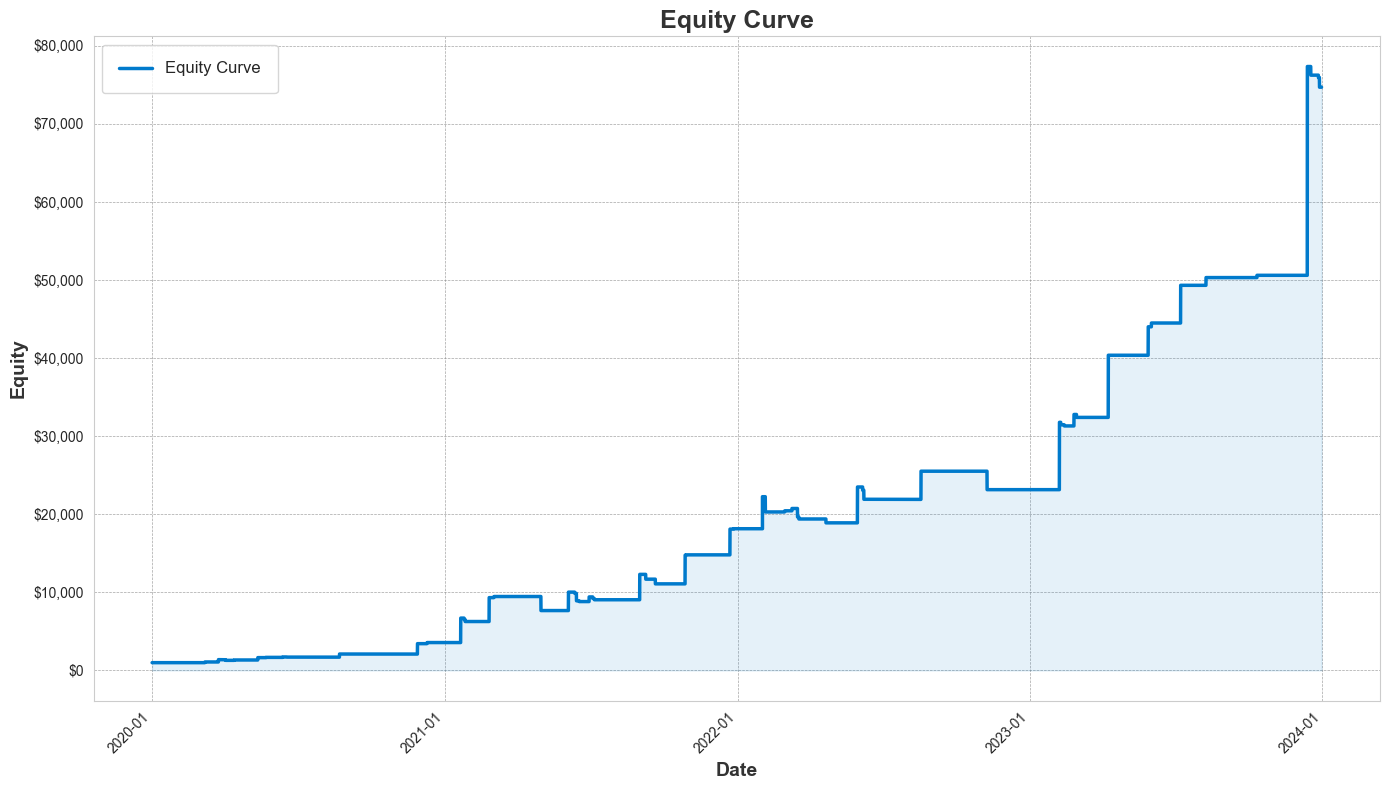
\includegraphics[width=\textwidth, height=2.2\textheight, keepaspectratio]{equity_mid.png} % Set image to full text width and increased height
    \vspace{1em} % Adds space between the image and the caption
    \caption{Bitcoin Equity.}
    \label{fig:sample-image} % Label for referencing the image in text
    \vspace{2\baselineskip} % Adds additional vertical space (2 lines) before the note
    \textit{Note: The fees have not been deducted from this calculation. After deducting fees, the final amount is expected to remain approximately the same.}
\end{figure}



\begin{figure}[htbp!] % 'h' option suggests here placement
    \centering
    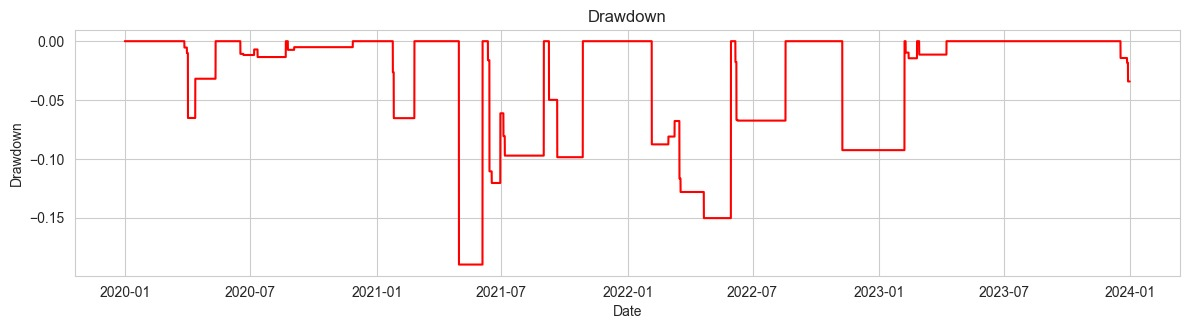
\includegraphics[width=\textwidth, height=2.2\textheight, keepaspectratio]{drawdown.jpg} % Set image to full text width and increased height
    \vspace{1em} % Adds space between the image and the caption
    \caption{Bitcoin Equity.}
    \label{fig:sample-image} % Label for referencing the image in text

  
\end{figure}

\newpage
\thispagestyle{empty}
\mbox{}


\thispagestyle{empty}
\section{Unique Approaches and Innovations}
\subsection{Unique or Innovative Aspects of the Strategy}
Our trading strategy integrates multiple advanced technical indicators, most notably Heikin-Ashi Candlesticks, MACD, EMA Crossovers, and ADX, which together provide a robust system for detecting market trends, momentum, and volatility. This multi-indicator approach seeks to exploit both trend-following and mean-reverting behaviors in the market, providing a well-rounded strategy for various market conditions.

\begin{itemize}
    \item \textbf{EMA:} Provides a more reliable confirmation of trends.
    \item \textbf{MACD with Heikin-Ashi:} Using MACD on Heikin-Ashi close prices smooths out price action, reducing false signals and enhancing accuracy in volatile markets.
    \item \textbf{ADX and Directional Indicators:} ADX, $+DI$, and $-DI$ help filter out weak trends, focusing trades only on strong, directional movements.
    \item \textbf{Risk Management with ATR:} ATR is used to set dynamic stop-loss (SL) and take-profit (TP) levels, adjusting to market volatility. This ensures better risk management and more adaptive position sizing, protecting against sudden volatility and locking in profits during strong trends.
\end{itemize}

\newpage

\subsection{How This Approach Differs from Traditional Methods of Trading}
Our approach is unique compared to traditional trading methods due to the following reasons:
\begin{itemize}
    \item \textbf{Combination of Multiple Indicators:} Many traditional trading strategies rely on one or two indicators to determine entry and exit points (such as using only RSI, MACD, or a single EMA). In contrast, our strategy combines several trend-following indicators (e.g., Triple EMA, ADX) and momentum indicators (e.g., MACD) to create a more comprehensive picture of the market.
    \item \textbf{Triple EMA System:} This offers a layered approach that allows for a finer-grained understanding of the market's momentum. Many traders use just one EMA, but we use multiple EMAs across different periods to smooth out short-term fluctuations while capturing longer-term trends.
    \item \textbf{Heikin-Ashi Candlesticks for Trend Confirmation:} Traditional trading strategies typically use regular candlesticks for market analysis. Our strategy employs Heikin-Ashi candlesticks, which help smooth out price action, making it easier to identify trends and eliminate noise.
    \item \textbf{Incorporation of Trend Strength (ADX):} Traditional methods often focus on trend direction without explicitly considering trend strength. By using ADX and the $+DI$/$-DI$ indicators, our strategy not only identifies whether a market is trending but also determines whether the trend is strong enough to warrant an entry.
    \item \textbf{Dynamic Risk Management with ATR:} Traditional trading strategies may use fixed stop-loss and take-profit levels. Our strategy uses ATR to dynamically adjust SL and TP levels according to market volatility, reducing the likelihood of getting stopped out in volatile conditions.
    \item \textbf{Volume Filtering:} The use of volume moving averages as a filter for entry signals helps eliminate false signals caused by low-volume trades, improving overall signal reliability.
\end{itemize}

\newpage
\section{Future Work: Transition Plan for Improving the Trading Algorithm}
As we move closer to the final round of the competition, we have identified certain areas where the current trading algorithm can be enhanced. The goal is to optimize performance, reduce drawdown, and increase overall profitability.



\subsection*{Future Improvements for Ethereum (ETH) Strategy}

Our current trading strategy on Ethereum (ETH) has been underperforming relative to our Bitcoin. In its current state, the ETH strategy lacks the robustness needed to achieve optimal returns and minimize drawdown effectively. 

\textbf{Planned Enhancements:}
As part of our future work, we will be dedicating significant efforts to develop and improve the ETH trading strategy. Our primary goals include:

\begin{itemize}
    \item \textbf{Strengthening Robustness:} By integrating additional indicators and refining our entry and exit logic, we aim to enhance the stability and adaptability of the ETH strategy in various market conditions.
    \item \textbf{Improving Final Balance:} We will focus on optimizing the strategy’s profitability through fine-tuning risk management techniques, such as dynamic stop-loss and take-profit levels.
    \item \textbf{Reducing Drawdown:} High drawdowns have impacted the ETH strategy's sustainability. To address this, we will work on adjusting position sizing, refining risk controls, and implementing volatility-based adjustments to keep drawdown levels within acceptable limits.
\end{itemize}

By prioritizing these enhancements, we expect to significantly improve the performance of our ETH strategy, aligning it with the robust standards set by other assets in our portfolio. Our goal is to achieve consistent returns with lower risk, making Ethereum trading a more valuable component of our overall strategy.




\subsection*{1. Objective: Minimize Drawdown While Maximizing Returns}
\textbf{Current Challenge:} The present algorithm yields a reasonable profit, but it suffers from a relatively high maximum drawdown.
\begin{itemize}
    \item \textbf{Solution:} We will refine the stop loss (SL) and take profit (TP) levels to better capture market movements with controlled risk, using ATR to adjust SL and TP levels based on market volatility.
    \item \textbf{Expected Outcome:} By optimizing SL/TP levels, we aim to increase profits while lowering the drawdown during high-volatility periods.
\end{itemize}

\subsection*{2. Incorporating Machine Learning for SL/TP Optimization}
\textbf{Current Challenge:} The strategy currently uses static SL and TP values.
\begin{itemize}
    \item \textbf{Solution:} Implement machine learning (ML) techniques to dynamically adjust SL and TP based on historical data, market patterns, and volatility measures.
    \item \textbf{Expected Outcome:} The ML optimization will enable more informed exit decisions, potentially improving the overall risk/reward profile.
\end{itemize}

\subsection*{3. Reducing Overfitting and Improving Generalization}
\textbf{Current Challenge:} The current strategy might be overfitted to historical data.
\begin{itemize}
    \item \textbf{Solution:} Apply regularization techniques (e.g., L2 regularization, dropout) and cross-validation, and select robust features (L1 regularization) and tune hyperparameters.
    \item \textbf{Expected Outcome:} A more flexible and robust strategy that performs consistently across different market conditions.
\end{itemize}

\subsection*{4. Improving Maximum Adverse Excursion (MAE)}
\textbf{Current Challenge:} The Maximum Adverse Excursion (MAE) has been higher than expected.
\begin{itemize}
    \item \textbf{Solution:} Reduce MAE by fine-tuning the entry and exit logic, using more responsive indicators like ADX and EMA crossovers.
    \item \textbf{Expected Outcome:} Minimized MAE, resulting in fewer large drawdowns and more efficient trades.
\end{itemize}

\subsection*{5. Reducing Maximum Drawdown (Max DD) and Improving Final Balance}
\textbf{Current Challenge:} The strategy shows promising returns, but the maximum drawdown remains high.
\begin{itemize}
    \item \textbf{Solution:} Explore risk management techniques such as dynamic position sizing and trailing stop orders.
    \item \textbf{Expected Outcome:} Improved risk-adjusted return and more stable growth in final balance.
\end{itemize}

\subsection*{6. Improving Quarterly Performance}
\textbf{Current Challenge:} Inconsistent quarterly results.
\begin{itemize}
    \item \textbf{Solution:} Analyze quarterly performance and adjust the strategy based on seasonality, market trends, and specific asset volatility.
    \item \textbf{Expected Outcome:} More balanced quarterly returns throughout the year.
\end{itemize}







\end{document}
